\documentclass[letterpaper, 12pt]{article} 
\usepackage[total={18cm,21cm},top=2cm, left=2cm]{geometry}
\parindent = 0mm % Sin sangr�a
\usepackage{latexsym,amsmath,amssymb,amsfonts}
\usepackage[latin1]{inputenc}
\usepackage[T1]{fontenc}
\usepackage{graphicx}
\usepackage[spanish]{babel} % Idioma espa�ol
\renewcommand{\baselinestretch}{1.1} % espaciado 1.1
\pagestyle{myheadings}
\markright{...... texto .......} % Encabezados simples
\usepackage{multicol}



\begin{document}

\parbox{9cm}{ 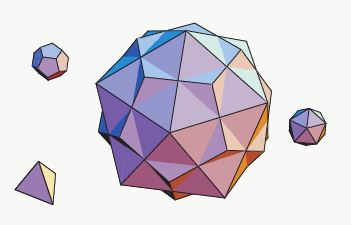
\includegraphics{images/1.jpg}} \parbox{9cm}{ En
{\sc Mathematica}, podemos eliminar una o varias caras de un dodecaedro,
seleccionar el color y el grosor de las aristas y poner color a las caras.
Para esto debemos utilizar los comandos ... } %Sale del 2do parbox!

\end{document}